\documentclass[tikz,border=8pt]{standalone}
\usepackage{tikz}
\usetikzlibrary{arrows.meta,positioning,calc,backgrounds,fit}
\usepackage[sfdefault]{inter}
\usepackage[T1]{fontenc}

% Colors (colorblind-safe)
\definecolor{speakerA}{HTML}{0072B2}
\definecolor{speakerB}{HTML}{E69F00}
\definecolor{visGreen}{HTML}{009E73}
\definecolor{hidRed}{HTML}{D55E00}
\definecolor{neutralGray}{HTML}{595959}
\definecolor{bandGray}{HTML}{F0F0F0}

\begin{document}
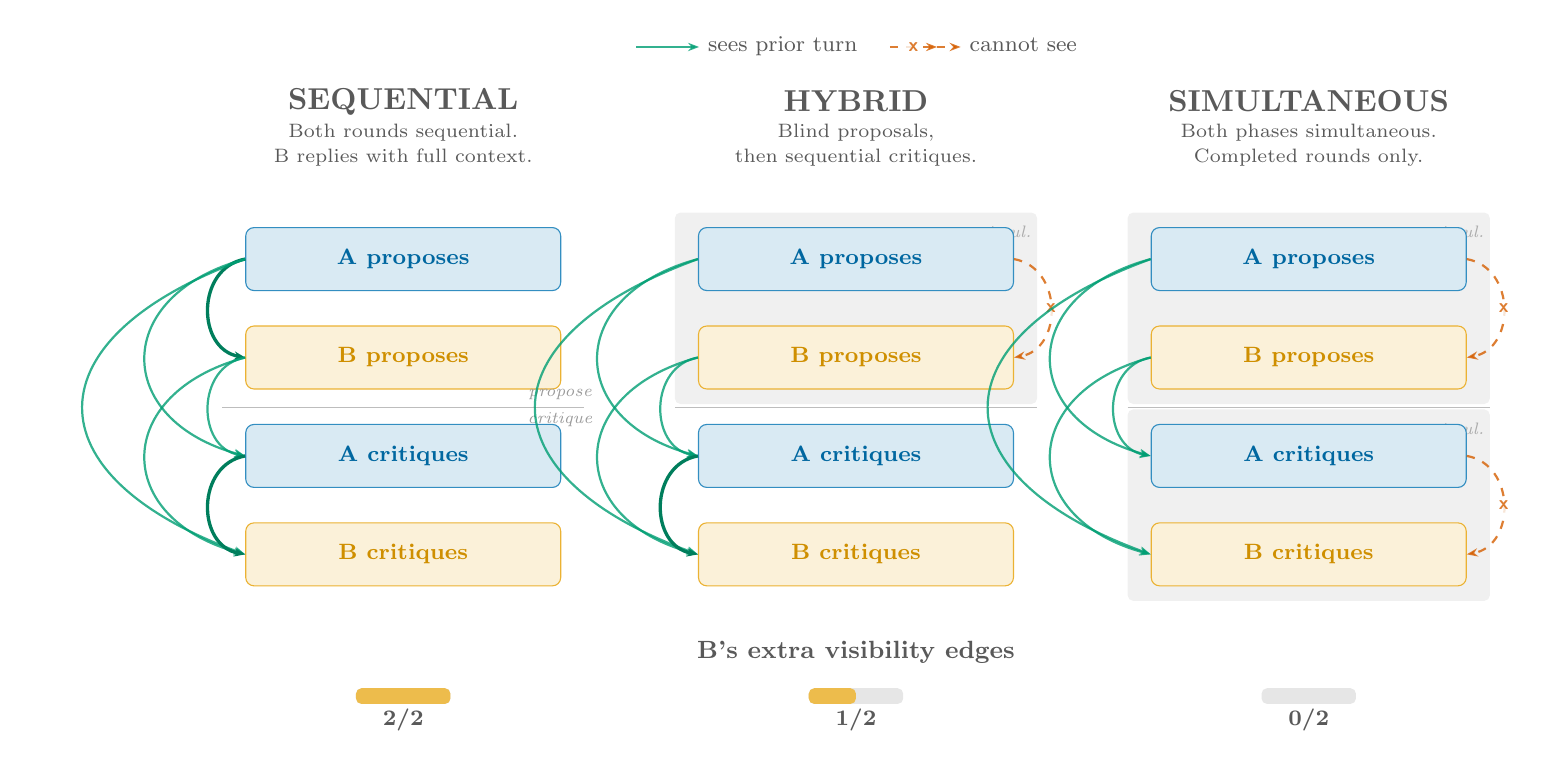
\begin{tikzpicture}[
    execute at begin node={\hyphenpenalty=10000\exhyphenpenalty=10000\tolerance=800},
    turnA/.style={
        draw=speakerA!80, fill=speakerA!15, text=speakerA!90!black,
        rounded corners=3pt, minimum width=4.0cm, minimum height=0.8cm,
        font=\fontsize{8.5}{10}\selectfont\bfseries, align=center
    },
    turnB/.style={
        draw=speakerB!80, fill=speakerB!15, text=speakerB!90!black,
        rounded corners=3pt, minimum width=4.0cm, minimum height=0.8cm,
        font=\fontsize{8.5}{10}\selectfont\bfseries, align=center
    },
    sees/.style={
        -{Stealth[length=4pt]}, visGreen, thick, opacity=0.8
    },
    seesKey/.style={
        -{Stealth[length=4pt]}, visGreen!80!black, very thick
    },
    hidden/.style={
        -{Stealth[length=4pt]}, hidRed, thick, dashed, opacity=0.8
    },
    header/.style={
        font=\fontsize{11}{13}\selectfont\bfseries, text=neutralGray
    },
    subtitle/.style={
        font=\fontsize{7.5}{9}\selectfont, text=neutralGray, align=center,
        text width=4.8cm
    },
    xmark/.style={
        fill=white, inner sep=1.5pt, font=\fontsize{7}{8}\selectfont\bfseries,
        text=hidRed
    },
    scorelabel/.style={
        font=\fontsize{8}{10}\selectfont, text=neutralGray
    },
]

% Column positions
\def\colA{0}
\def\colB{5.75}
\def\colC{11.50}

% Y positions
\def\yHeader{0}
\def\ySub{-0.55}
\def\yNote{-1.15}
\def\yA{-2.0}
\def\yBp{-3.25}
\def\yAc{-4.5}
\def\yBc{-5.75}
\def\yScore{-7.0}

% ===== Legend (top center) =====
\node[scorelabel] at (5.75, 0.7) {%
    \tikz[baseline=-0.5ex]{
        \draw[sees] (0,0) -- (0.8,0);
    } sees prior turn \quad
    \tikz[baseline=-0.5ex]{
        \draw[hidden] (0,0) -- (0.6,0) node[midway, xmark]{\textsf{x}};
        \draw[hidden] (0.6,0) -- (0.9,0);
    } cannot see
};

% ===== SEQUENTIAL =====
\begin{scope}[xshift=\colA cm]
    \node[header] at (0, \yHeader) {SEQUENTIAL};
    \node[subtitle] at (0, \ySub) {Both rounds sequential.\\B replies with full context.};

    \node[turnA] (sA1) at (0, \yA)  {A proposes};
    \node[turnB] (sB2) at (0, \yBp) {B proposes};
    \node[turnA] (sA3) at (0, \yAc) {A critiques};
    \node[turnB] (sB4) at (0, \yBc) {B critiques};

    % Visibility arrows (left side = sees)
    \draw[seesKey] (sA1.west) to[out=190, in=170, looseness=1.3] (sB2.west);
    \draw[sees] (sA1.west) to[out=195, in=165, looseness=1.8] (sA3.west);
    \draw[sees] (sB2.west) to[out=190, in=170, looseness=1.3] (sA3.west);
    \draw[sees] (sA1.west) to[out=200, in=160, looseness=2.0] (sB4.west);
    \draw[sees] (sB2.west) to[out=195, in=165, looseness=1.8] (sB4.west);
    \draw[seesKey] (sA3.west) to[out=190, in=170, looseness=1.3] (sB4.west);

    % Phase separator
    \draw[neutralGray!40, thin] (-2.3, -3.88) -- (2.3, -3.88);
    \node[font=\fontsize{6.5}{8}\selectfont, text=neutralGray!60] at (2.0, -3.72) {\textit{propose}};
    \node[font=\fontsize{6.5}{8}\selectfont, text=neutralGray!60] at (2.0, -4.04) {\textit{critique}};
\end{scope}

% ===== HYBRID =====
\begin{scope}[xshift=\colB cm]
    \node[header] at (0, \yHeader) {HYBRID};
    \node[subtitle] at (0, \ySub) {Blind proposals,\\then sequential critiques.};

    % Simultaneous band for propose
    \begin{pgfonlayer}{background}
        \node[fill=bandGray, rounded corners=2pt, inner sep=4pt,
              fit={($(0,-1.55)$) ($(0,-3.7)$)},
              minimum width=4.6cm] {};
        \node[font=\fontsize{6}{7}\selectfont, text=neutralGray!50]
              at (1.9, -1.65) {\textit{simul.}};
    \end{pgfonlayer}

    \node[turnA] (hA1) at (0, \yA)  {A proposes};
    \node[turnB] (hB2) at (0, \yBp) {B proposes};
    \node[turnA] (hA3) at (0, \yAc) {A critiques};
    \node[turnB] (hB4) at (0, \yBc) {B critiques};

    % Hidden: A1 -> B2 (can't see)
    \draw[hidden] (hA1.east) to[out=-10, in=10, looseness=1.3]
        node[midway, xmark]{\textsf{x}} (hB2.east);

    % Visible
    \draw[sees] (hA1.west) to[out=195, in=165, looseness=1.8] (hA3.west);
    \draw[sees] (hB2.west) to[out=190, in=170, looseness=1.3] (hA3.west);
    \draw[sees] (hA1.west) to[out=200, in=160, looseness=2.0] (hB4.west);
    \draw[sees] (hB2.west) to[out=195, in=165, looseness=1.8] (hB4.west);
    \draw[seesKey] (hA3.west) to[out=190, in=170, looseness=1.3] (hB4.west);

    % Phase separator
    \draw[neutralGray!40, thin] (-2.3, -3.88) -- (2.3, -3.88);
\end{scope}

% ===== SIMULTANEOUS =====
\begin{scope}[xshift=\colC cm]
    \node[header] at (0, \yHeader) {SIMULTANEOUS};
    \node[subtitle] at (0, \ySub) {Both phases simultaneous.\\Completed rounds only.};

    % Simultaneous bands
    \begin{pgfonlayer}{background}
        \node[fill=bandGray, rounded corners=2pt, inner sep=4pt,
              fit={($(0,-1.55)$) ($(0,-3.7)$)},
              minimum width=4.6cm] {};
        \node[font=\fontsize{6}{7}\selectfont, text=neutralGray!50]
              at (1.9, -1.65) {\textit{simul.}};
        \node[fill=bandGray, rounded corners=2pt, inner sep=4pt,
              fit={($(0,-4.05)$) ($(0,-6.2)$)},
              minimum width=4.6cm] {};
        \node[font=\fontsize{6}{7}\selectfont, text=neutralGray!50]
              at (1.9, -4.15) {\textit{simul.}};
    \end{pgfonlayer}

    \node[turnA] (tA1) at (0, \yA)  {A proposes};
    \node[turnB] (tB2) at (0, \yBp) {B proposes};
    \node[turnA] (tA3) at (0, \yAc) {A critiques};
    \node[turnB] (tB4) at (0, \yBc) {B critiques};

    % Hidden: A1 -> B2
    \draw[hidden] (tA1.east) to[out=-10, in=10, looseness=1.3]
        node[midway, xmark]{\textsf{x}} (tB2.east);
    % Hidden: A3 -> B4
    \draw[hidden] (tA3.east) to[out=-10, in=10, looseness=1.3]
        node[midway, xmark]{\textsf{x}} (tB4.east);

    % Visible
    \draw[sees] (tA1.west) to[out=195, in=165, looseness=1.8] (tA3.west);
    \draw[sees] (tB2.west) to[out=190, in=170, looseness=1.3] (tA3.west);
    \draw[sees] (tA1.west) to[out=200, in=160, looseness=2.0] (tB4.west);
    \draw[sees] (tB2.west) to[out=195, in=165, looseness=1.8] (tB4.west);

    % Phase separator
    \draw[neutralGray!40, thin] (-2.3, -3.88) -- (2.3, -3.88);
\end{scope}

% ===== B's Information Advantage Score =====
\node[font=\fontsize{9}{11}\selectfont\bfseries, text=neutralGray]
    at (5.75, \yScore) {B's extra visibility edges};

% Score bars
\foreach \col/\score/\label in {\colA/2/2, \colB/1/1, \colC/0/0} {
    \begin{scope}[xshift=\col cm]
        % Background segments
        \fill[neutralGray!15, rounded corners=2pt] (-0.6, \yScore-0.45) rectangle (0.6, \yScore-0.65);
        % Filled segments
        \ifnum\score>0
            \fill[speakerB!70, rounded corners=2pt] (-0.6, \yScore-0.45) rectangle ({-0.6+1.2*\score/2}, \yScore-0.65);
        \fi
        \node[font=\fontsize{8}{10}\selectfont\bfseries, text=neutralGray]
            at (0, \yScore-0.85) {\label/2};
    \end{scope}
}

\end{tikzpicture}
\end{document}
